\section{特別課題}
\subsection{Mandelbrot 集合}
\begin{figure}[htbp]
  \centering
  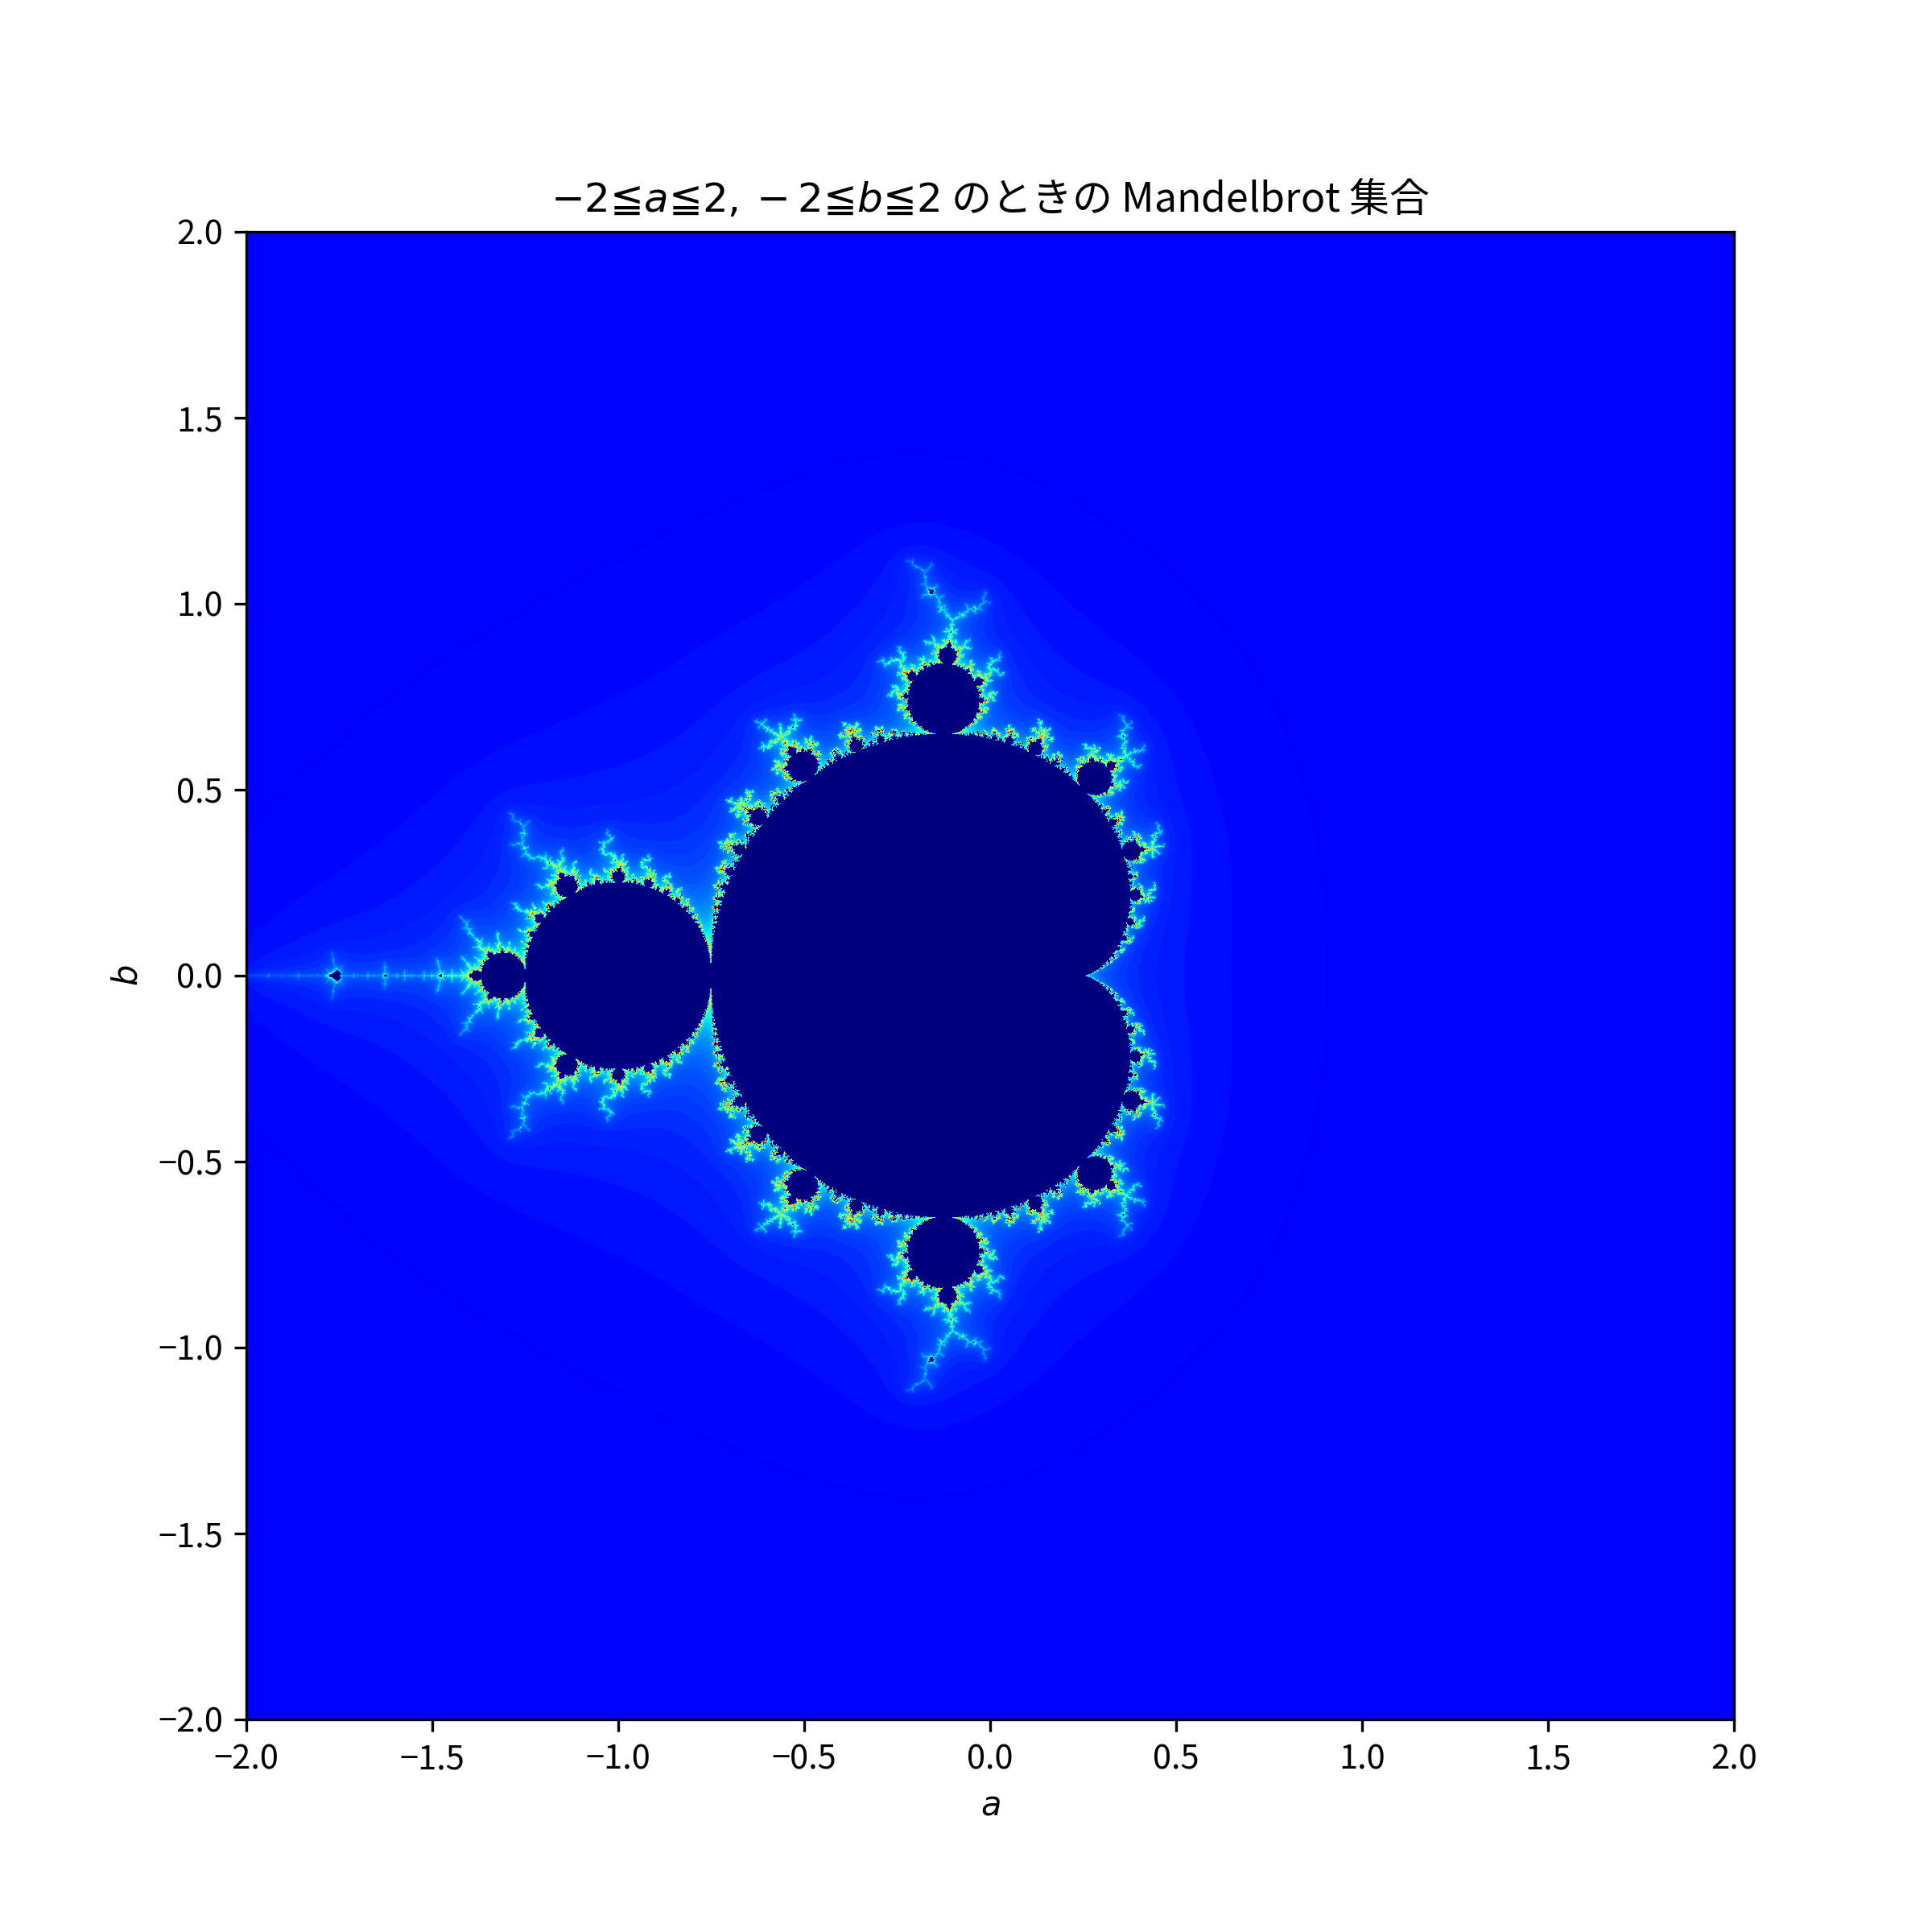
\includegraphics[keepaspectratio, scale=0.8]{images/OtherProblem/ctest5_1.png}
\end{figure}
解説:\\
今回はPythonを用いて複素数の計算を簡略化しマンデルブロ集合をプロットした。まず、$a, b$ それぞれの範囲での漸化式を計算し、それを複素数平面上にプロットした。\\
\begin{lstlisting}[caption=mandelbrot.py]
  import numpy as np
  import matplotlib
  from matplotlib import pyplot as plt
  from matplotlib.colors import Normalize                     # カラーマップを自在に操作するために必要
  from numba import jit                                       # 計算の高速化


  # 日本語フォント用(Linux)
  matplotlib.rc('font', family='Noto Sans CJK JP')
  '''
  # 日本語フォント用(Windows)
  matplotlib.rc('font', family='MS Gothic')
  '''

  @jit
  def mandelbrot(a, b, n_max):
      "複素数を用いてマンデルブロ集合の座標を求める関数"
      a_num, b_num = np.meshgrid(a, b)
      n_grid = len(a_num.ravel())                             # 組み合わせの総数
      z = np.zeros(n_grid)                                    # マンデルブロ集合のデータ格納用空配列


      for i in range(n_grid):
          c = complex(a_num.ravel()[i], b_num.ravel()[i])     # c = a + bi
          n = 0
          z0 = complex(0, 0)
          while np.abs(z0) < np.inf and not n == n_max:
              z0 = z0 ** 2 + c                                # 漸化式を計算
              n += 1
          
          if n == n_max:
              z[i] = 0
          else:
              z[i] = n
      z = np.reshape(z, a_num.shape)                          # 2次元配列に変換
      z = z[::-1]                                             # imshow()で上下逆になるので上下反転
      return z


  a = np.linspace(-2, 2, 2000)
  b = np.linspace(-2, 2, 2000)
  z = mandelbrot(a, b, 100)
  file_path = "複雑系科学演習/Week6/images/"
  plt.figure(figsize=(8, 8))
  plt.xlabel('$a$')
  plt.ylabel('$b$')
  plt.title("$-2 \leqq a \leqq 2, -2 \leqq b \leqq 2$ のときの Mandelbrot 集合")
  plt.imshow(z, cmap='jet', norm=Normalize(vmin=0, vmax=100), extent=[-2, 2, -2, 2])
  plt.savefig(file_path + "ctest5_1", dpi=300)
  plt.show()
\end{lstlisting}

\newpage
\subsection{Julia 集合}
\begin{figure}[htbp]
  \centering
  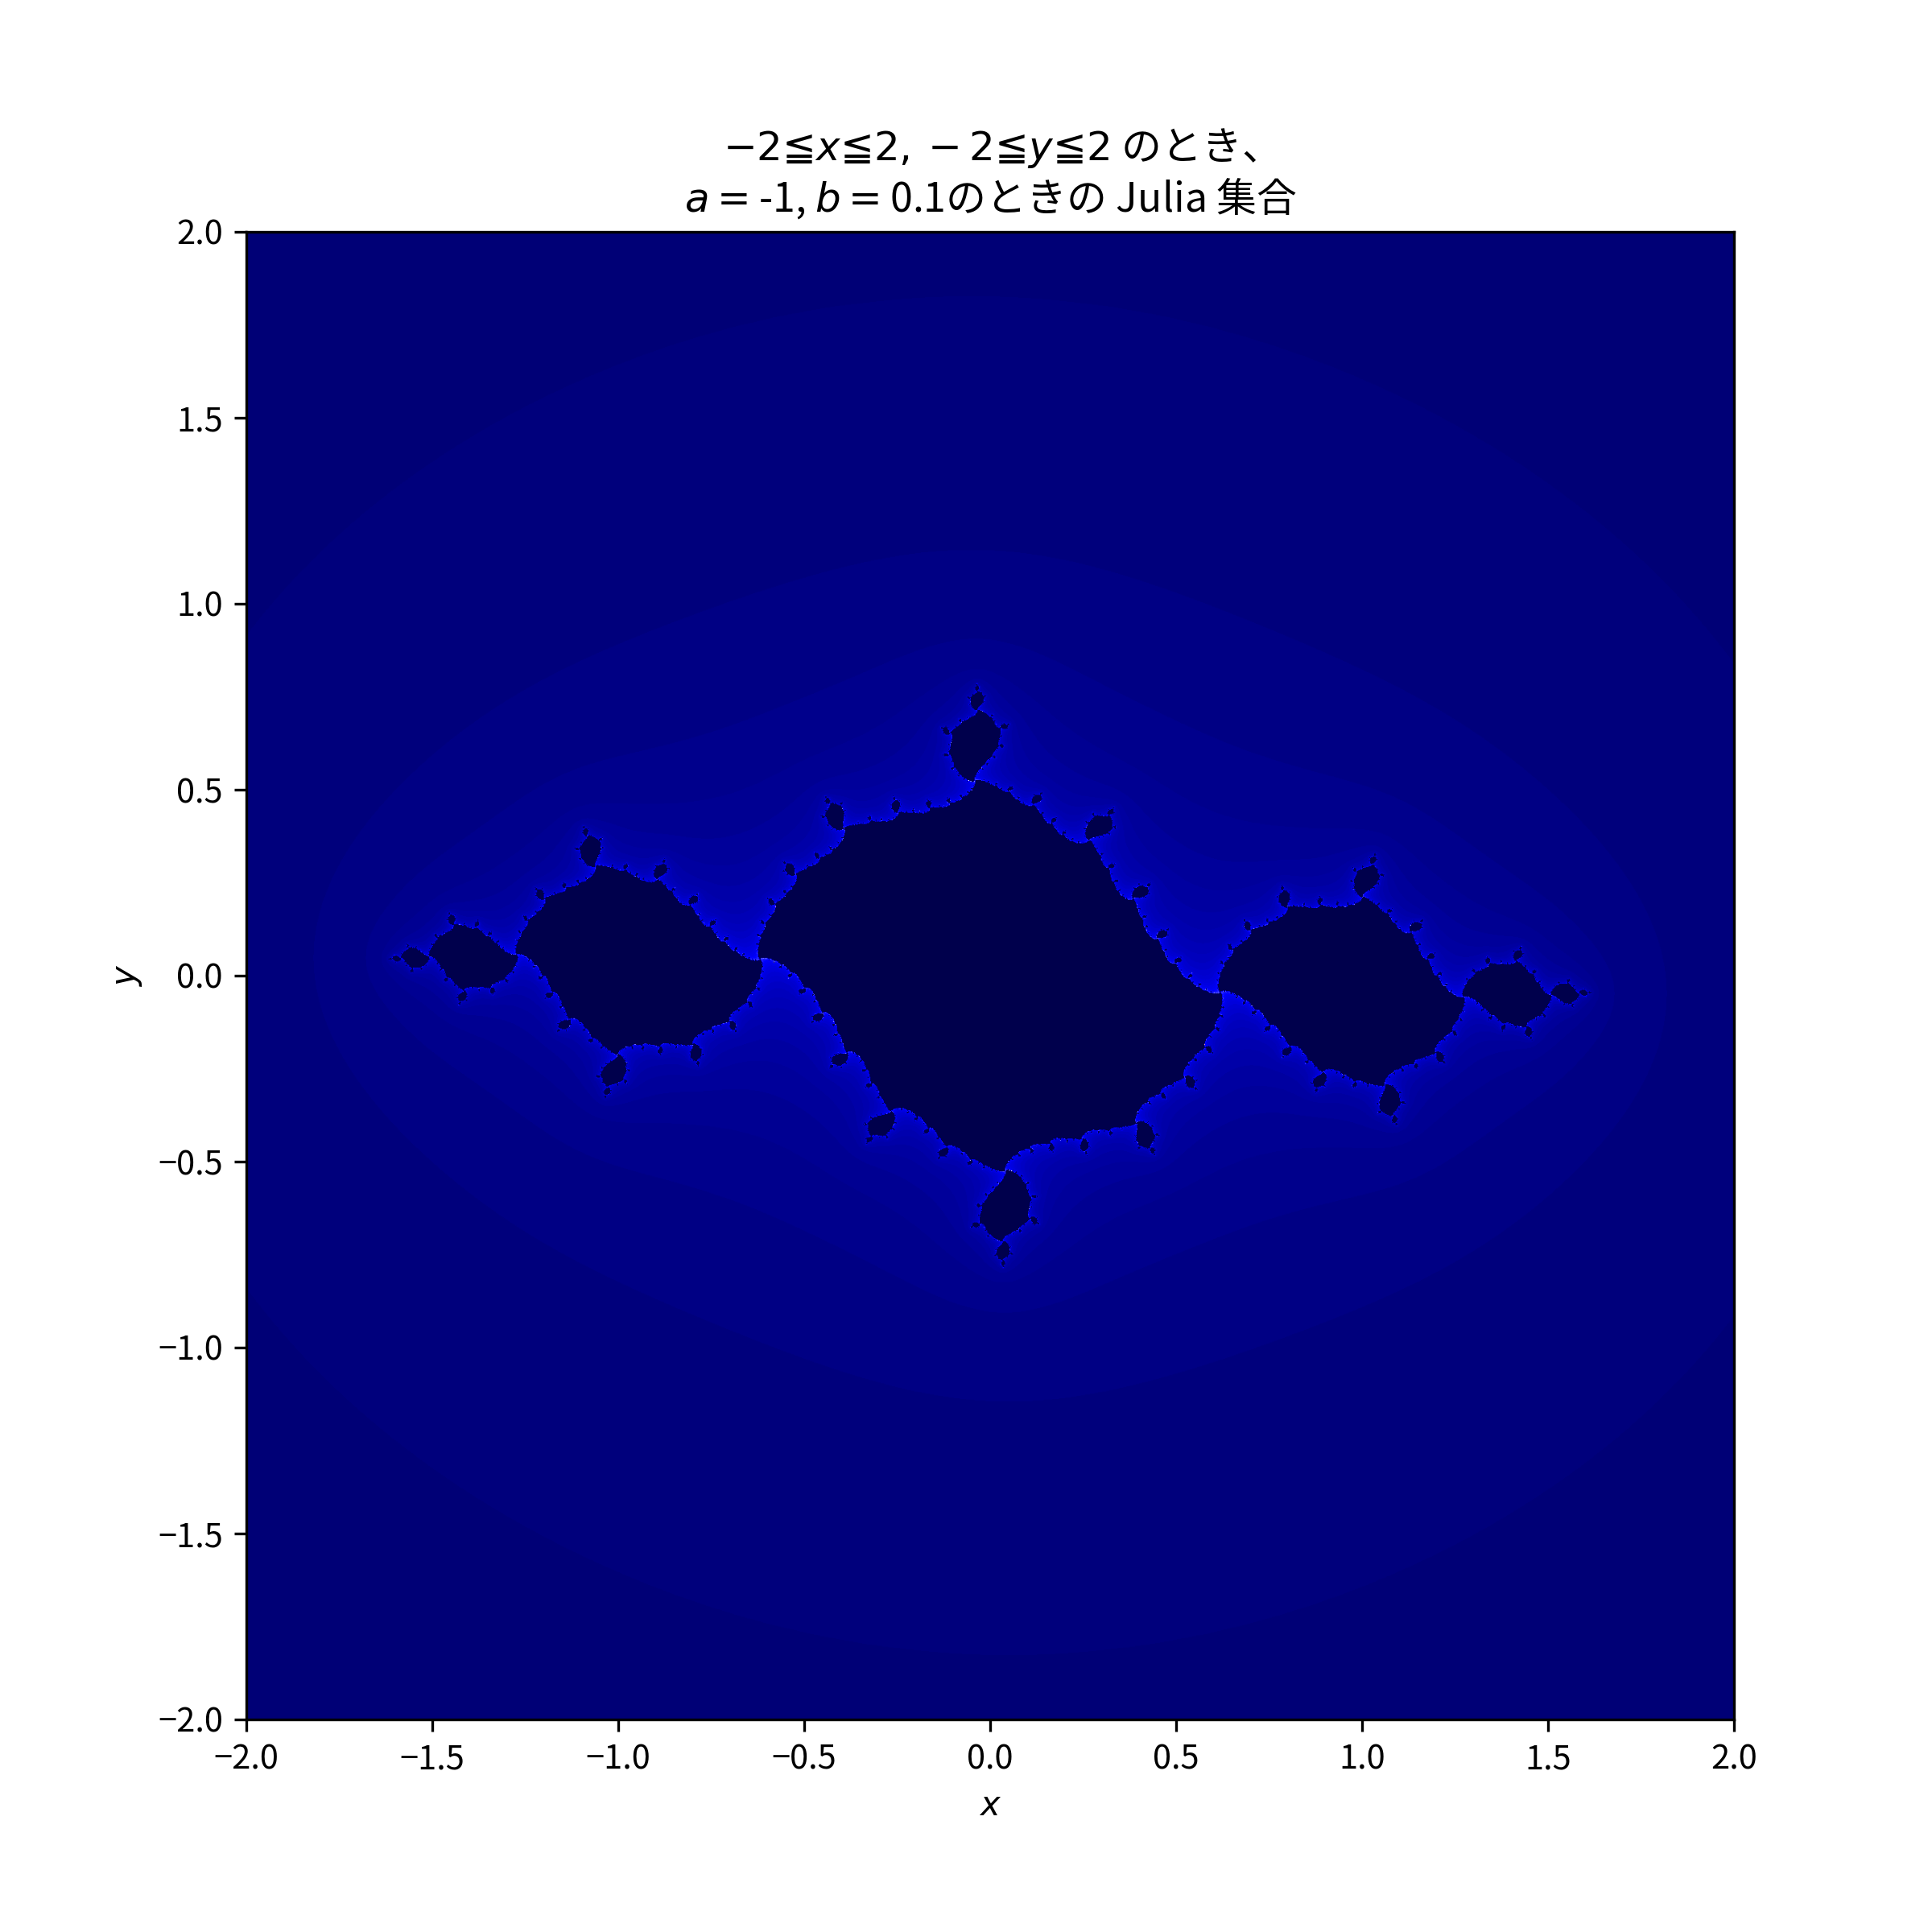
\includegraphics[keepaspectratio, scale=0.8]{images/OtherProblem/ctest5_2.png}
\end{figure}
解説:\\
ジュリア集合はマンデルブロ集合と似たような集合である。マンデルブロ集合では、$z_0 = 0$ として $c$ を変化させてきたがジュリア集合は逆の $c$ を固定し $z_0$ を変化させていく集合である。\\
\begin{lstlisting}[caption=julia.py]
  import numpy as np
  from matplotlib import pyplot as plt
  from matplotlib.colors import Normalize                 # カラーマップ操作
  from numba import jit                                   # 計算の高速化
  from random import uniform
  import matplotlib

  # 日本語フォント用(Linux)
  matplotlib.rc('font', family='Noto Sans CJK JP')
  '''
  # 日本語フォント用(Windows)
  matplotlib.rc('font', family='MS Gothic')
  '''

  @jit                                                    # 計算の高速化
  def julia(x, y, n_max, a, b):
      x_num, y_num = np.meshgrid(x, y)                    # xとyの組み合わせを計算
      n_grid = len(x_num.ravel())                         # 組み合わせの総数
      z = np.zeros(n_grid)                                # ジュリア集合のデータ格納用空配列

      for i in range(n_grid):
          c = complex(a, b)                               # c = a + bi

          n = 0
          z0 = complex(x_num.ravel()[i], y_num.ravel()[i])

          while np.abs(z0) < 1e20 and not n == n_max:
              z0 = z0 ** 2 + c                            # 漸化式を計算
              n += 1
          if n == n_max:
              z[i] = 0
          else:
              z[i] = n
      z = np.reshape(z, x_num.shape)                      # 2次元配列(画像表示用)に変換
      z = z[::-1]                                         # imshow()で上下逆になるので上下反転
      return z


  x = np.linspace(-2, 2, 2000)
  y = np.linspace(-2, 2, 2000)
  n_max = 100

  a = -1
  b = 0.1
  z = julia(x, y, n_max, a, b)
  file_path = "複雑系科学演習/Week6/images/"
  plt.figure(figsize=(8, 8))
  plt.xlabel('$x$')
  plt.ylabel('$y$')
  plt.title("$-2 \leqq x \leqq 2, -2 \leqq y \leqq 2$ のとき、\n" +\
      "$a = ${0}, $b = ${1}のときの Julia 集合".format(round(a, 3), round(b, 3)))

  plt.imshow(z, cmap='seismic', norm=Normalize(vmin=0, vmax=n_max), extent=[-2, 2, -2, 2])
  plt.savefig(file_path + "ctest5_2", dpi=300)
  plt.show()
\end{lstlisting}

\newpage
\subsection{Koch 曲線}
\begin{figure}[htbp]
  \centering
  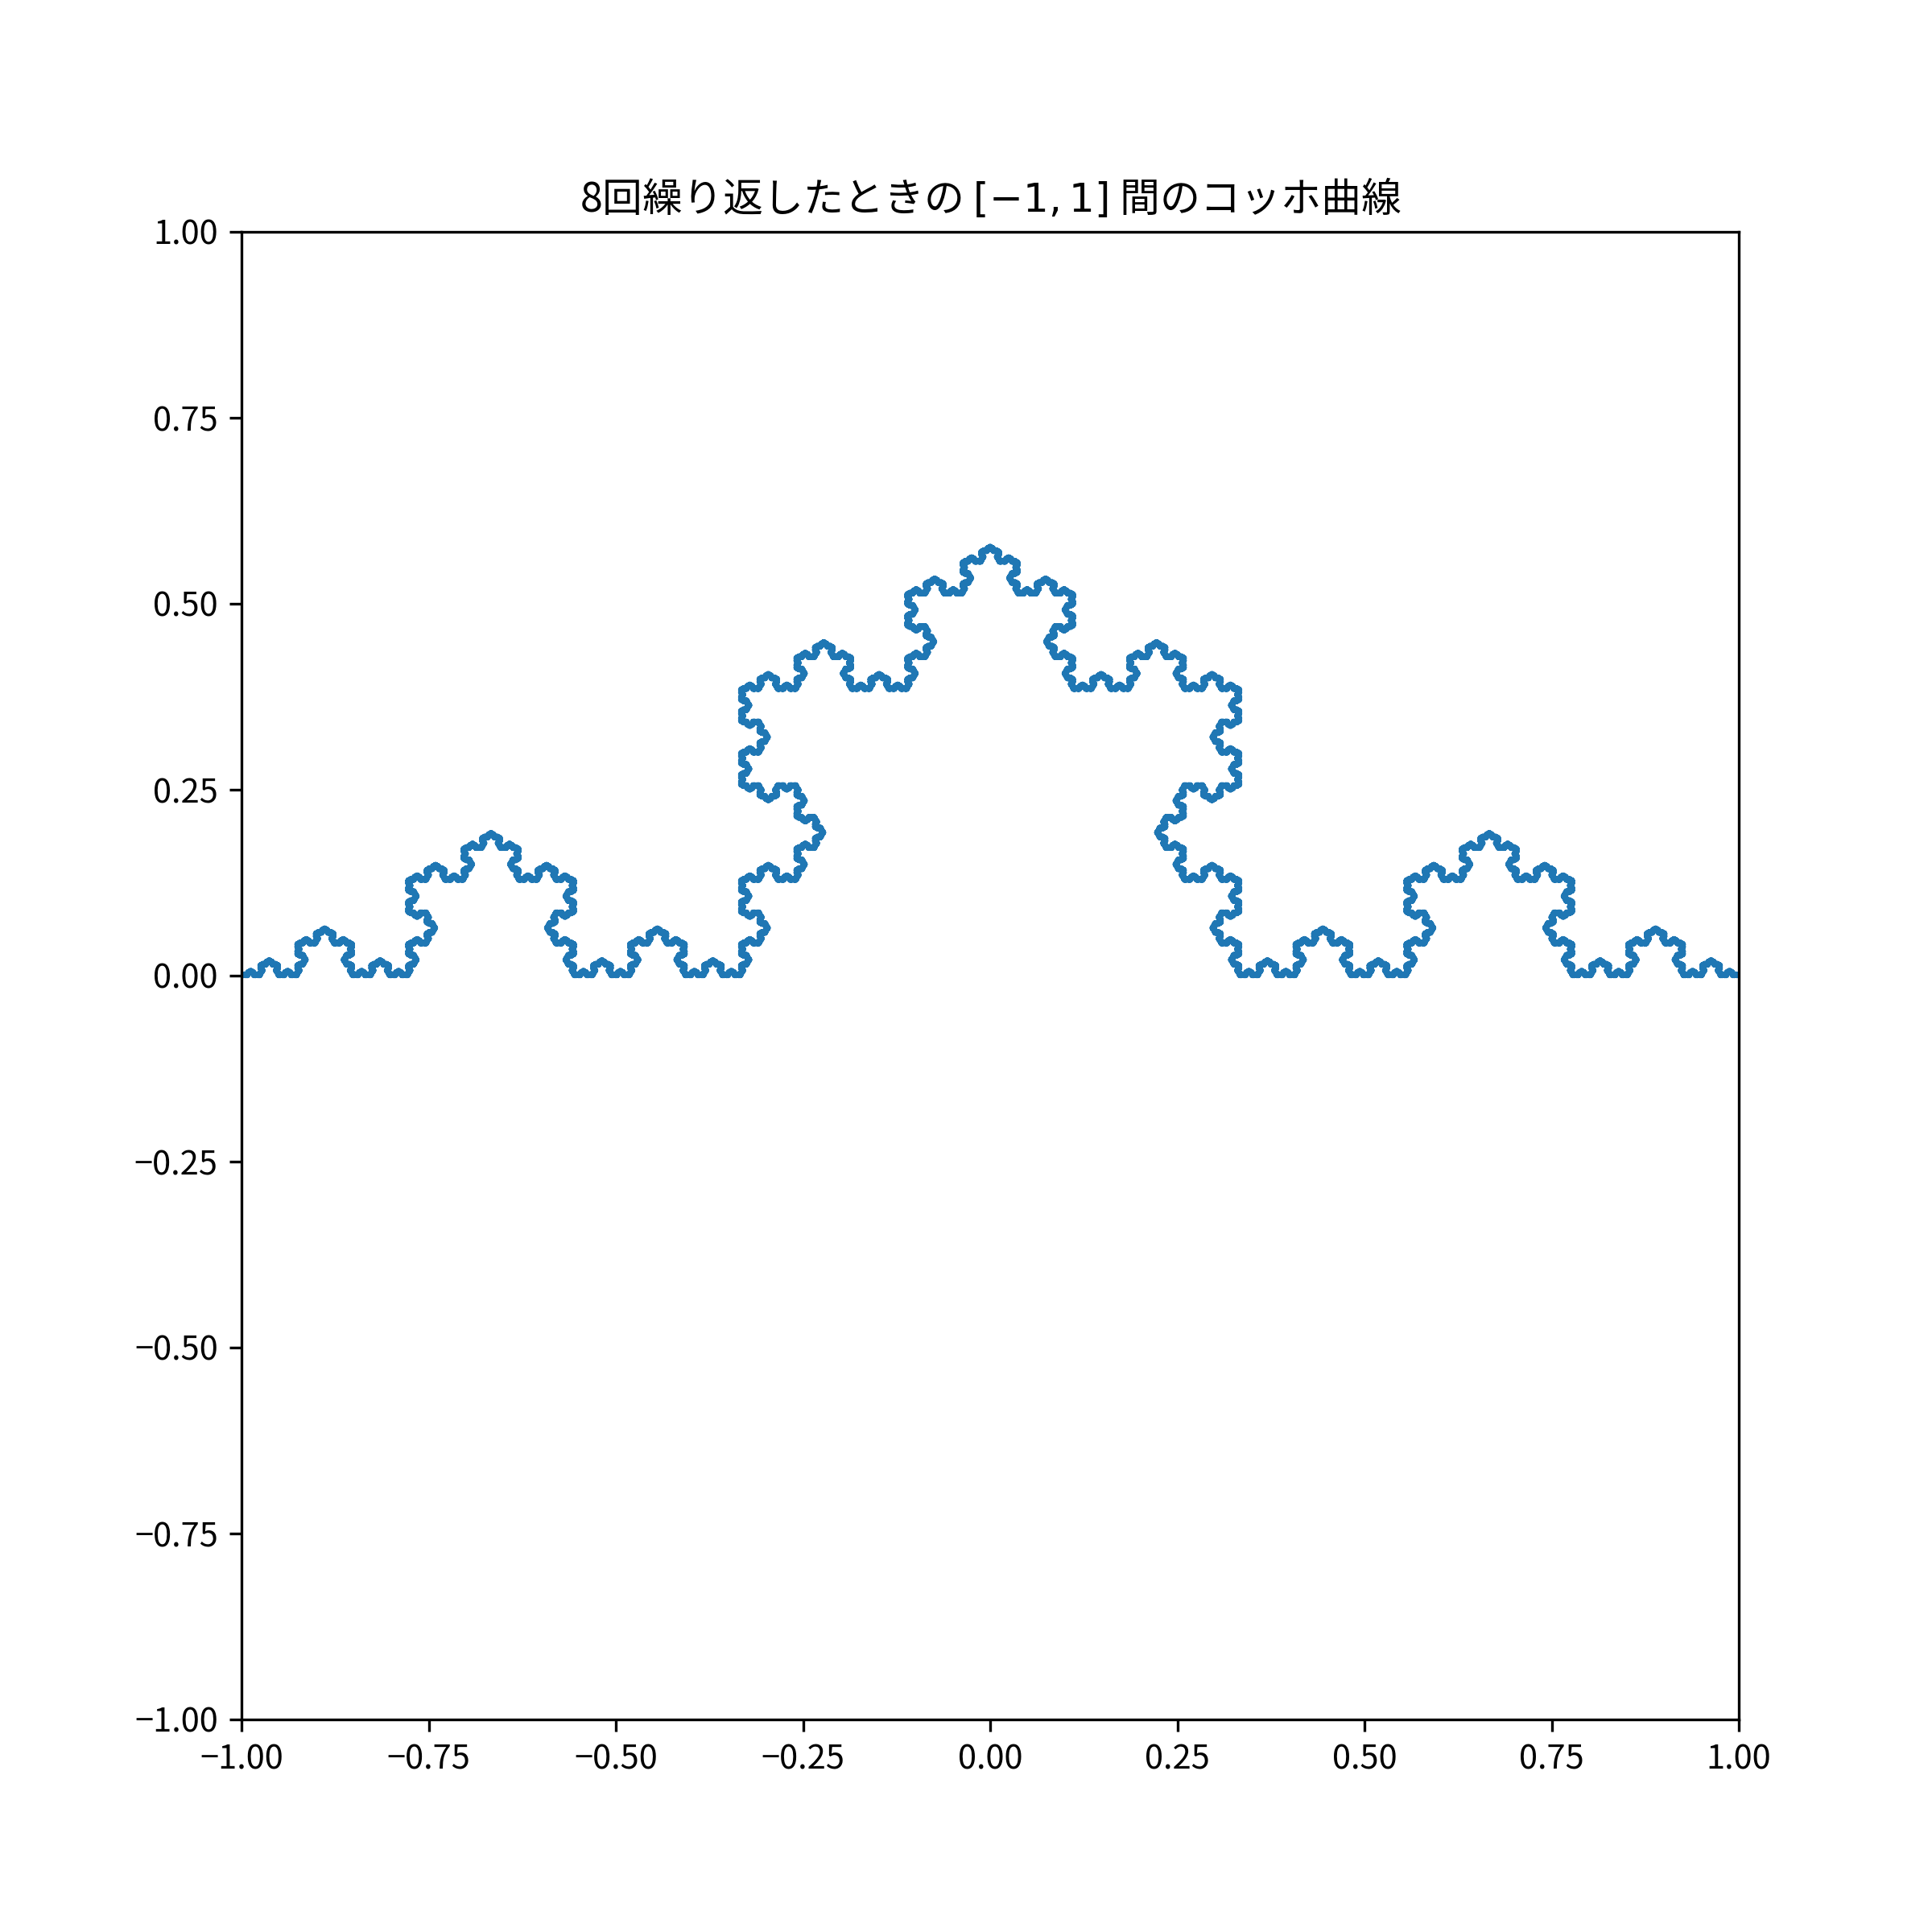
\includegraphics[keepaspectratio, scale=0.8]{images/OtherProblem/ctest5_3.png}
\end{figure}
解説:\\
このコッホ曲線を描くためのソースコードは、コッホ曲線の座標を任意の繰り返し回数で再帰し求める関数を作った。その座標の配列をもとにPythonのmatplotlibを用いてプロットした。\\
\begin{lstlisting}[caption=koch.py]
  import math
  import matplotlib
  from matplotlib import pyplot as plt
  import numpy as np

  # 日本語フォント用(Linux)
  matplotlib.rc('font', family='Noto Sans CJK JP')
  '''
  # 日本語フォント用(Windows)
  matplotlib.rc('font', family='MS Gothic')
  '''

  def koch(n: int, p1: list, p2: list) -> None:
      "再帰関数をもちいたコッホ曲線の座標を求める関数"
      if n == 0:
          return
      sx = 2 * p1[0] / 3 + p2[0] / 3
      sy = 2 * p1[1] / 3 + p2[1] / 3
      tx = p1[0] / 3 + 2 * p2[0] / 3
      ty = p1[1] / 3 + 2 * p2[1] / 3
      ux = (tx - sx) * math.cos(math.radians(60))  - (ty - sy) * math.sin(math.radians(60)) + sx
      uy = (tx - sx) * math.sin(math.radians(60)) + (ty - sy) * math.cos(math.radians(60)) + sy
      koch(n-1, p1, [sx, sy])
      # print(sx, sy)
      koch_array_x.append(sx)
      koch_array_y.append(sy)

      koch(n-1, [sx, sy], [ux, uy])
      # print(ux, uy)
      koch_array_x.append(ux)
      koch_array_y.append(uy)

      koch(n-1, [ux, uy], [tx, ty])
      # print(tx, ty)
      koch_array_x.append(tx)
      koch_array_y.append(ty)

      koch(n-1, [tx, ty], p2)

  n = 8
  p1 = [-1, 0]
  p2 = [1, 0]
  koch_array_x = [p1[0]]
  koch_array_y = [p1[1]]
  koch(n, p1, p2)
  koch_array_x.append(p2[0])
  koch_array_y.append(p2[1])
  file_path = "複雑系科学演習/Week6/images/"
  plt.figure(figsize=(8, 8))
  plt.title("{}回繰り返したときの $[-1, 1]$ 間のコッホ曲線".format(n))
  plt.xlim(-1, 1)
  plt.ylim(-1, 1)
  plt.plot(koch_array_x, koch_array_y)
  plt.savefig(file_path + "ctest5_3", dpi=300)
  plt.show()
\end{lstlisting}